\begin{frame}{a note on error checking}
\begin{itemize}
\item from pthread\_create manpage:
\end{itemize}
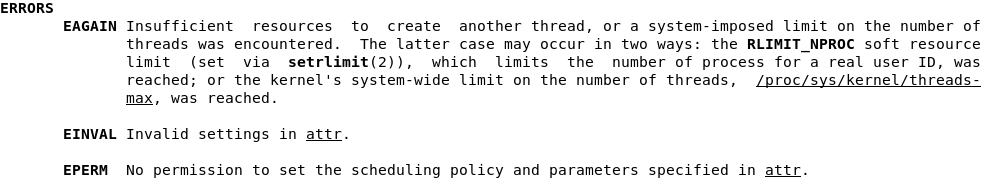
\includegraphics[width=\textwidth]{../threads/pthread-create-errors}
\begin{itemize}
\item special constants for \textit{return value}
\vspace{.5cm}
\item same pattern for many other pthreads functions
    \begin{itemize}
    \item pthread\_join, pthread\_mutex\_\ldots (later), \ldots
    \end{itemize}
\item will often omit error checking in slides for brevity
\end{itemize}
\end{frame}

\begin{frame}[fragile,label=pthreadCreateErrorCheck]{error checking pthread\_create}
\begin{lstlisting}[language=C++,style=small]
int error = pthread_create(...);
if (error != 0) {
    /* print some error message */
}
\end{lstlisting}
\end{frame}
